\documentclass[11pt,a4paper]{article}
\usepackage[margin=1in]{geometry}
\usepackage[T1]{fontenc}
\usepackage[utf8]{inputenc}
\usepackage{lmodern}
\usepackage{setspace}
\usepackage{booktabs}
\usepackage{longtable}
\usepackage{array}
\usepackage{graphicx}
\usepackage{float}
\usepackage{caption}
\usepackage{subcaption}
\usepackage{hyperref}
\usepackage{amsmath}
\usepackage{siunitx}
\usepackage{xcolor}
\usepackage{enumitem}
\setlist{nosep}
\onehalfspacing

\title{COMP0082 Coursework Report --- Protein Enzyme Classification}
\author{}
\date{March 2026}

\begin{document}
\maketitle

\section{Introduction}
Enzymes are biological catalysts that underpin virtually every metabolic process in living organisms.
The Enzyme Commission (EC) numbering system classifies enzymes into six top-level classes---
Oxidoreductases (EC 1), Transferases (EC 2), Hydrolases (EC 3), Lyases (EC 4),
Isomerases (EC 5), and Ligases (EC 6)---according to the reaction they catalyse.
Computational prediction of enzyme class from amino acid sequence alone is of substantial practical
importance: it accelerates the functional annotation of the millions of uncharacterised proteins
generated by high-throughput sequencing, and it supports drug target identification,
metabolic engineering, and synthetic biology.

This project addresses the problem as a seven-class supervised classification task, where class 0
represents \textit{Not an enzyme} and classes 1--6 correspond to the six EC classes.
The dataset comprises 39,764 non-homologous protein sequences with a heavily skewed distribution:
class 0 constitutes 81.5\% of the data, while the smallest class (Ligase, EC 6) accounts for only 0.7\%.
This extreme class imbalance is the central challenge of the project and informs every design decision,
from loss weighting and oversampling strategies to the choice of evaluation metrics.

\begin{table}[H]
\centering
\caption{Dataset class distribution.}
\begin{tabular}{lrr}
\toprule
Class & Label & Count \\
\midrule
0 & Not an enzyme & 32410 \\
1 & Oxidoreductase & 1184 \\
2 & Transferase & 2769 \\
3 & Hydrolase & 2108 \\
4 & Lyase & 600 \\
5 & Isomerase & 411 \\
6 & Ligase & 282 \\
\bottomrule
\end{tabular}
\end{table}

\begin{figure}[H]
\centering
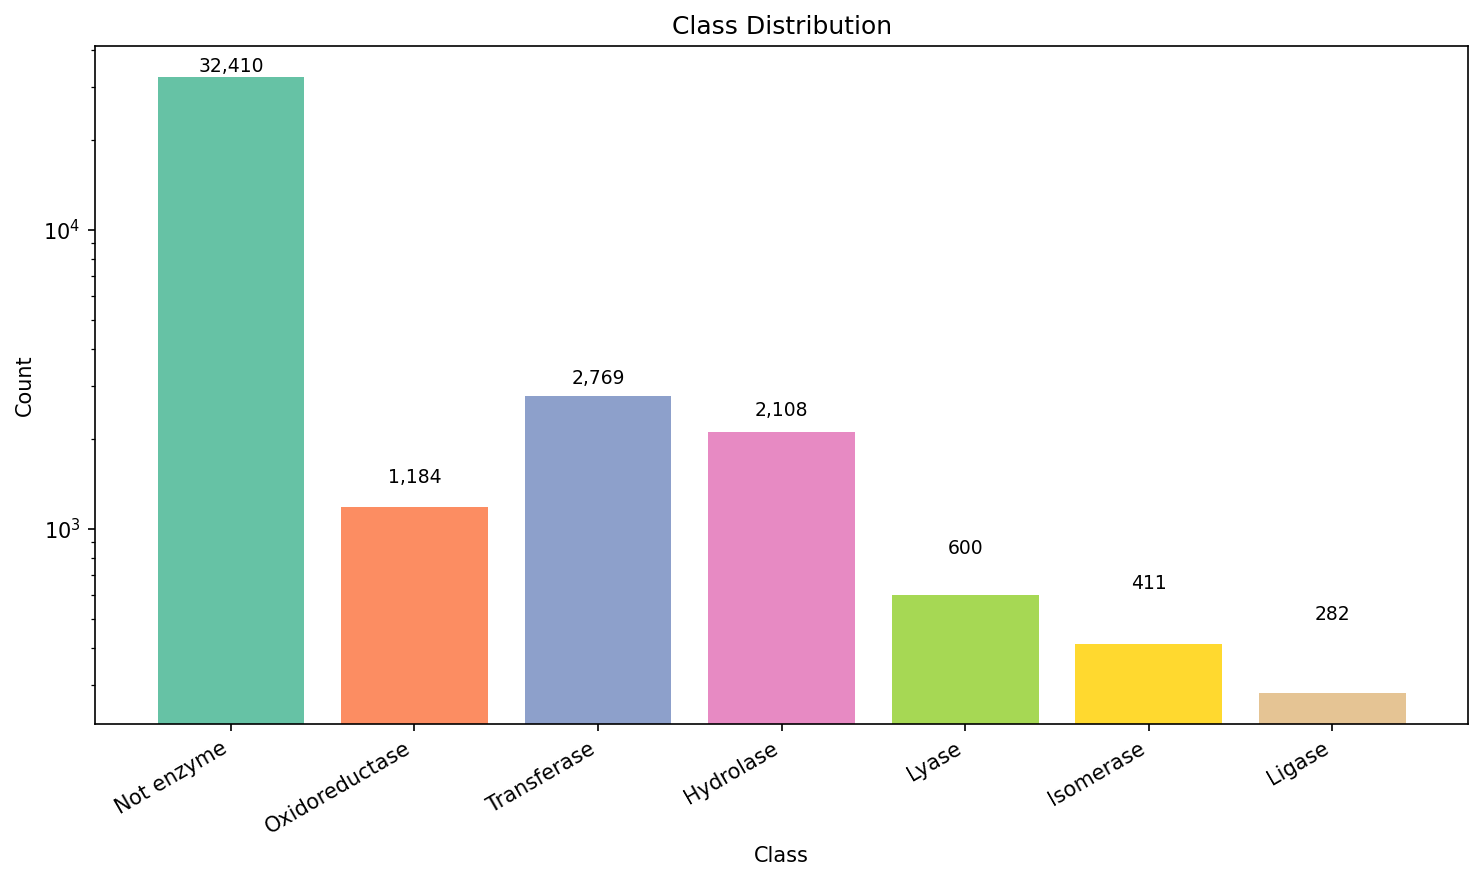
\includegraphics[width=0.78\textwidth]{../figures/class_distribution.png}
\caption{Observed class imbalance in the training dataset.}
\end{figure}

\section{Methods}
\subsection{Feature Engineering}
\textbf{Amino acid composition (20-d).} The normalised frequency of each canonical amino acid,
capturing global residue distribution.

\textbf{Dipeptide frequencies (400-d).} Normalised counts of all ordered amino acid pairs,
encoding local sequential context that single-residue composition cannot capture.
Combined with a sequence-length scalar, this yields a 421-dimensional handcrafted composition vector.

\textbf{Physicochemical properties (8-d).} Molecular weight, isoelectric point, aromaticity,
GRAVY hydropathicity, charge at pH 7.0, and Chou--Fasman secondary-structure propensity fractions
(helix, turn, sheet), computed using BioPython ProtParam.

\textbf{Protein language model embeddings.} ESM-2 was used as a feature extractor.
Two model sizes were evaluated: \texttt{esm2\_t6\_8M\_UR50D} (320-d) and
\texttt{esm2\_t33\_650M\_UR50D} (1,280-d).
Final-layer hidden states were mean-pooled across non-special tokens.

\subsection{Experimental Design}
All experiments used stratified 5-fold cross-validation (seed 42).
Leakage prevention rules were enforced:
\begin{enumerate}
\item Fold indices generated before feature normalisation.
\item \texttt{StandardScaler.fit()} on training fold only.
\item SMOTE on training fold only.
\item Features derived only from amino acid sequence.
\item Precomputed ESM embeddings treated as stateless features; normalisation still fold-local.
\end{enumerate}

Metrics: Accuracy, Macro F1, Balanced Accuracy, MCC.
Macro F1 was the primary model-selection criterion.

\subsection{Models}
\textbf{Baselines:} Logistic Regression (balanced class weights) and Random Forest variants on handcrafted features.

\textbf{Advanced models:} XGBoost and LightGBM on ESM-2 650M + physicochemical features (1,288-d), with and without SMOTE.

\textbf{Fine-tuning:} End-to-end ESM-2 8M fine-tuning with classification head
$\mathrm{Linear}(320,128) \to \mathrm{GELU} \to \mathrm{Dropout}(0.3) \to \mathrm{Linear}(128,7)$,
AdamW differential learning rates, OneCycleLR, mixed precision, gradient accumulation, early stopping.

\textbf{Ensemble:} Soft-vote blend of out-of-fold probabilities from fine-tuned 8M and XGBoost+SMOTE 650M.
Weights were proportional to each model's OOF Macro F1.

\section{Results}
\subsection{Model Comparison}
Table~\ref{tab:model-comparison} reports stratified 5-fold CV performance.
The final Ensemble row uses the generated OOF blend metrics from
\texttt{outputs/ensemble\_results.json}.

\begin{table}[H]
\centering
\caption{Model comparison (mean $\pm$ std for CV models; ensemble from OOF blend).}
\label{tab:model-comparison}
\begin{tabular}{lcccc}
\toprule
Model & Accuracy & Macro F1 & Bal. Acc. & MCC \\
\midrule
Logistic Regression & $0.457 \pm 0.003$ & $0.191 \pm 0.002$ & $0.300 \pm 0.010$ & $0.171 \pm 0.003$ \\
Random Forest & $0.816 \pm 0.001$ & $0.141 \pm 0.002$ & $0.149 \pm 0.001$ & $0.093 \pm 0.011$ \\
RF + PCA(50) & $0.816 \pm 0.002$ & $0.197 \pm 0.002$ & $0.185 \pm 0.001$ & $0.216 \pm 0.006$ \\
XGBoost & $0.886 \pm 0.003$ & $0.575 \pm 0.013$ & $0.516 \pm 0.011$ & $0.621 \pm 0.010$ \\
LightGBM & $0.879 \pm 0.003$ & $0.515 \pm 0.013$ & $0.467 \pm 0.008$ & $0.605 \pm 0.010$ \\
LightGBM + SMOTE & $0.880 \pm 0.002$ & $0.576 \pm 0.014$ & $0.535 \pm 0.010$ & $0.620 \pm 0.006$ \\
XGBoost + SMOTE & $0.886 \pm 0.002$ & $0.595 \pm 0.014$ & $0.552 \pm 0.011$ & $0.631 \pm 0.006$ \\
ESM-2 8M Fine-tune & $0.823 \pm 0.008$ & $0.509 \pm 0.013$ & $0.570 \pm 0.015$ & $0.553 \pm 0.008$ \\
\textbf{Ensemble (OOF)} & \textbf{0.890} & \textbf{0.625} & \textbf{0.605} & \textbf{0.659} \\
\bottomrule
\end{tabular}
\end{table}

\begin{figure}[H]
\centering
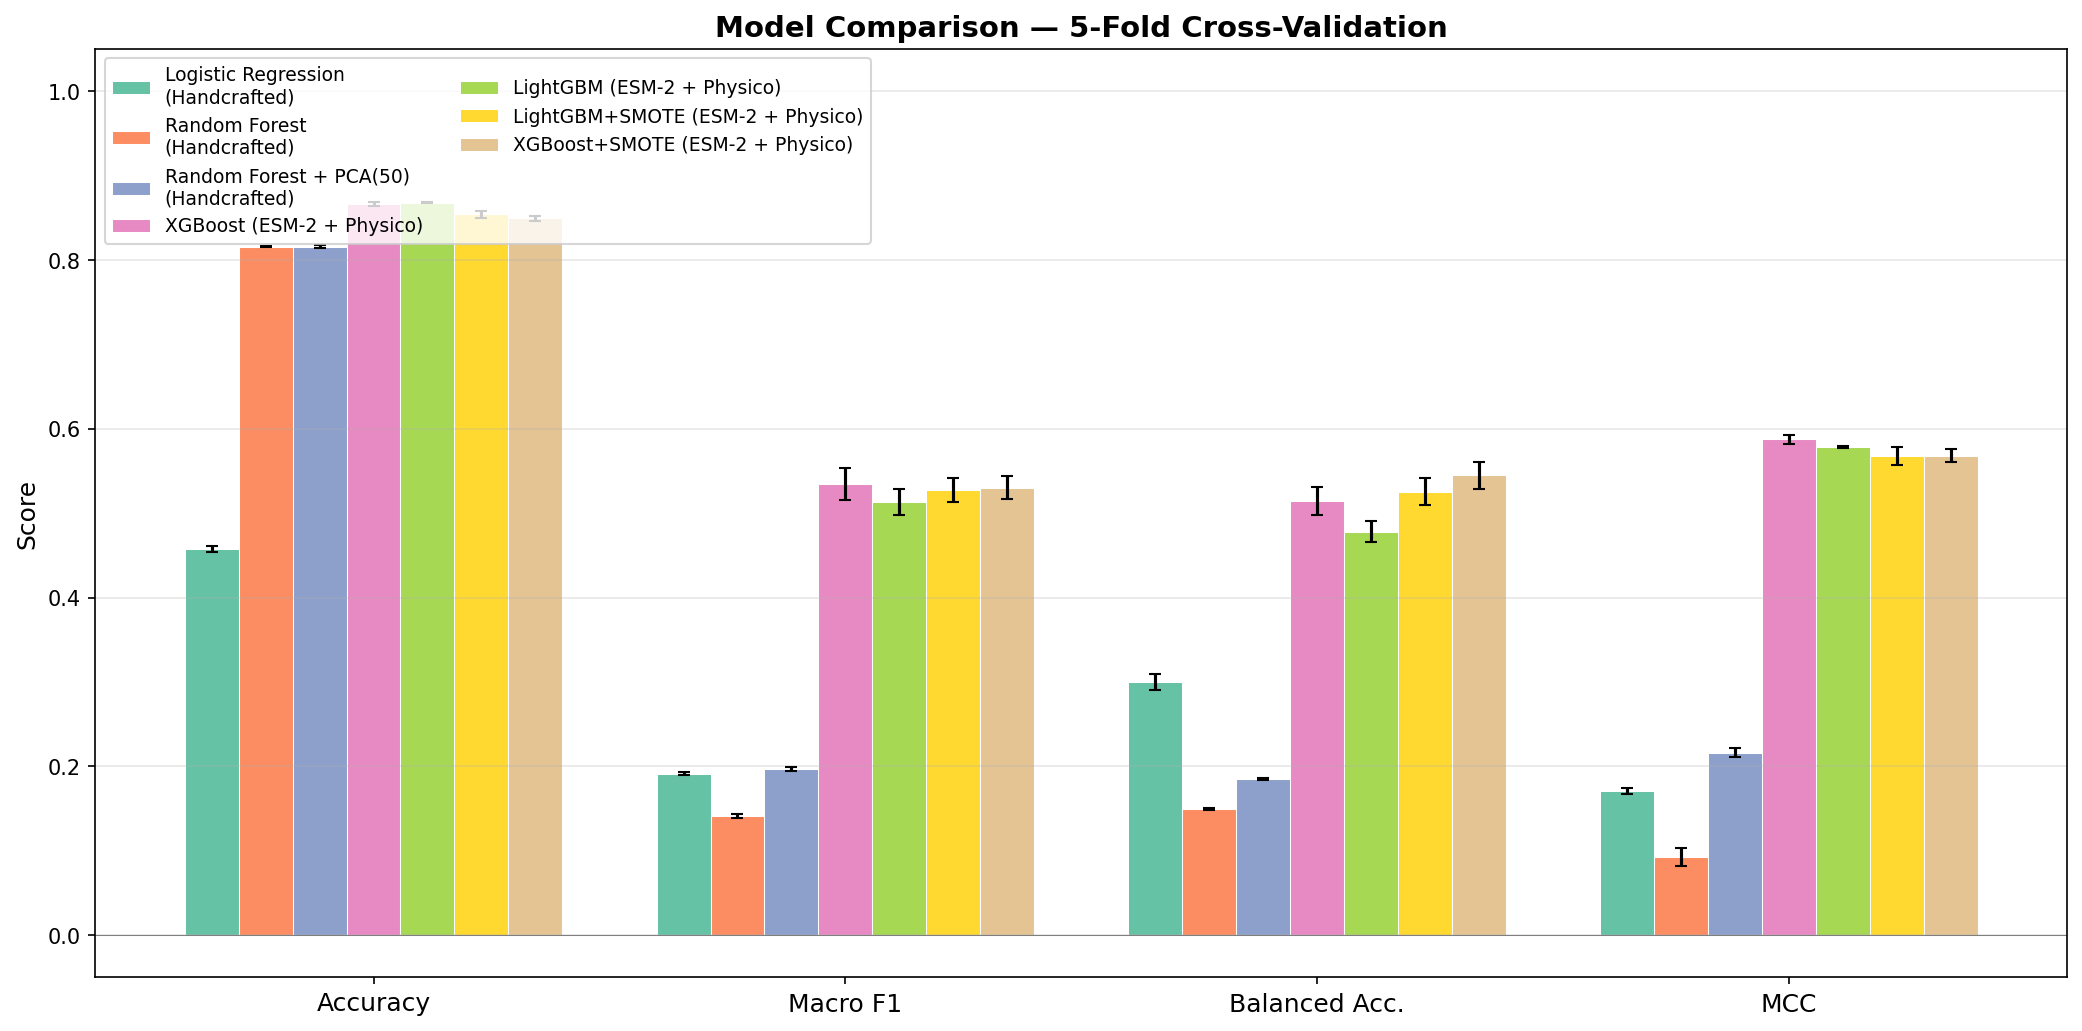
\includegraphics[width=0.88\textwidth]{../figures/model_comparison.png}
\caption{Aggregate comparison across major models.}
\end{figure}

\subsection{Feature Ablation}
\begin{table}[H]
\centering
\caption{Feature ablation study (XGBoost, balanced weights).}
\begin{tabular}{lcc}
\toprule
Feature Set & Dimensions & Macro F1 \\
\midrule
Handcrafted only & 429 & 0.206 \\
ESM-2 only & 1280 & 0.562 \\
ESM-2 + Handcrafted & 1709 & 0.552 \\
ESM-2 + Physicochemical & 1288 & 0.575 \\
\bottomrule
\end{tabular}
\end{table}

\begin{figure}[H]
\centering
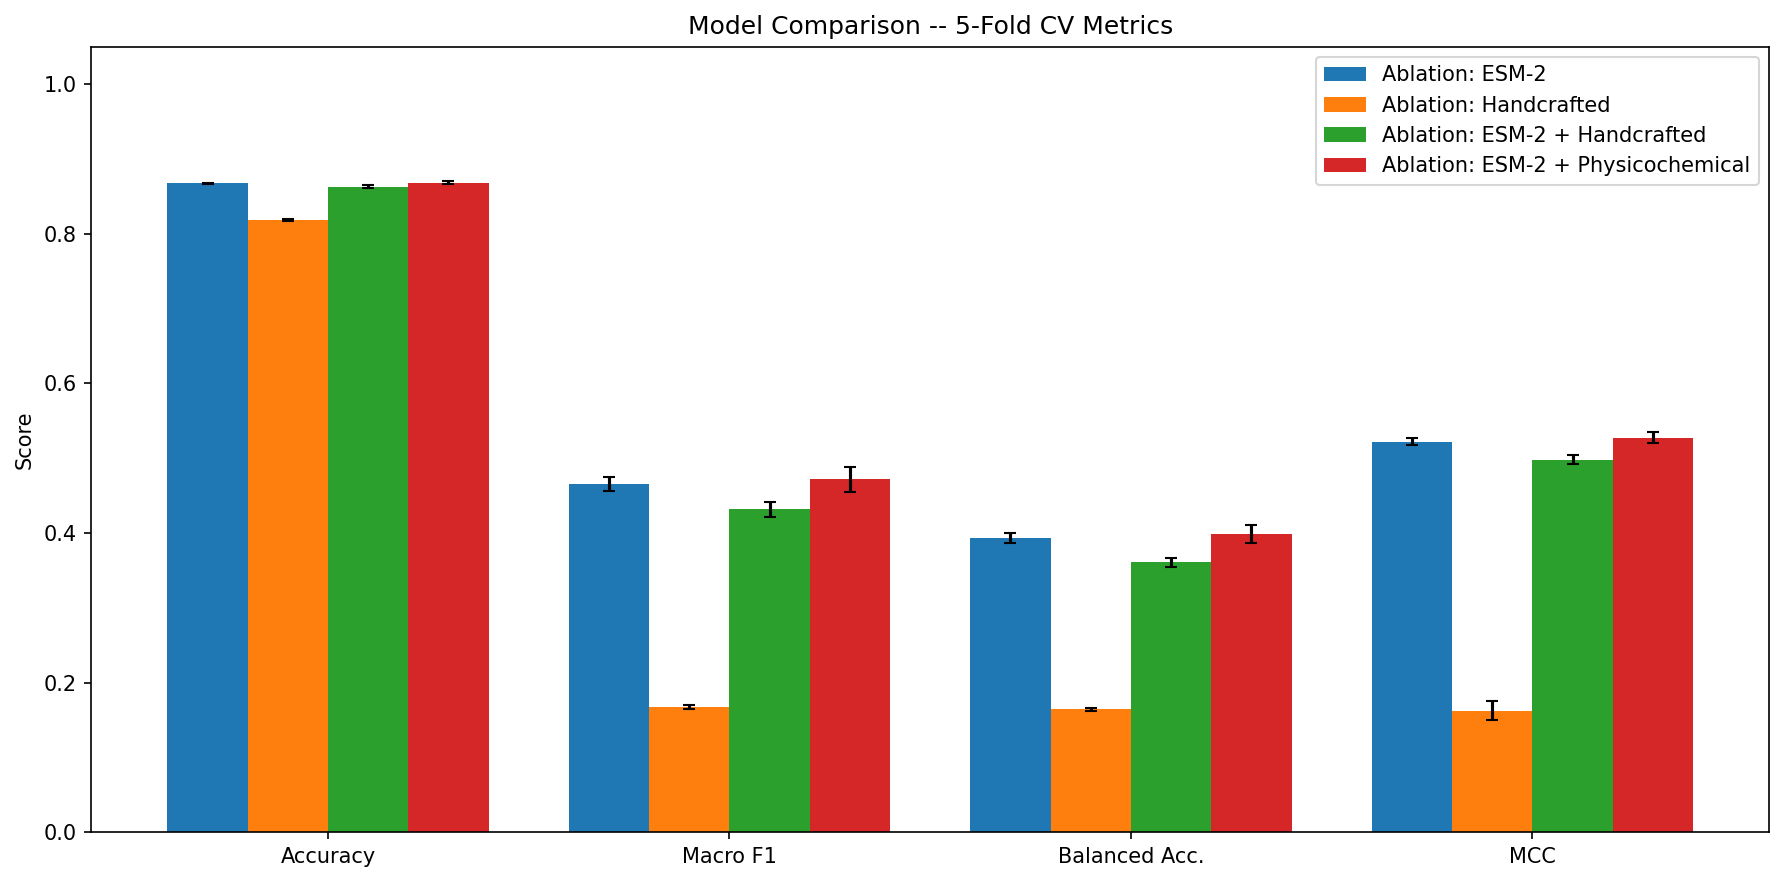
\includegraphics[width=0.72\textwidth]{../figures/ablation_results.png}
\caption{Ablation results showing dominant contribution of ESM-2 representations.}
\end{figure}

\subsection{Confusion Matrix Analysis}
\begin{figure}[H]
\centering
\begin{subfigure}{0.48\textwidth}
\centering
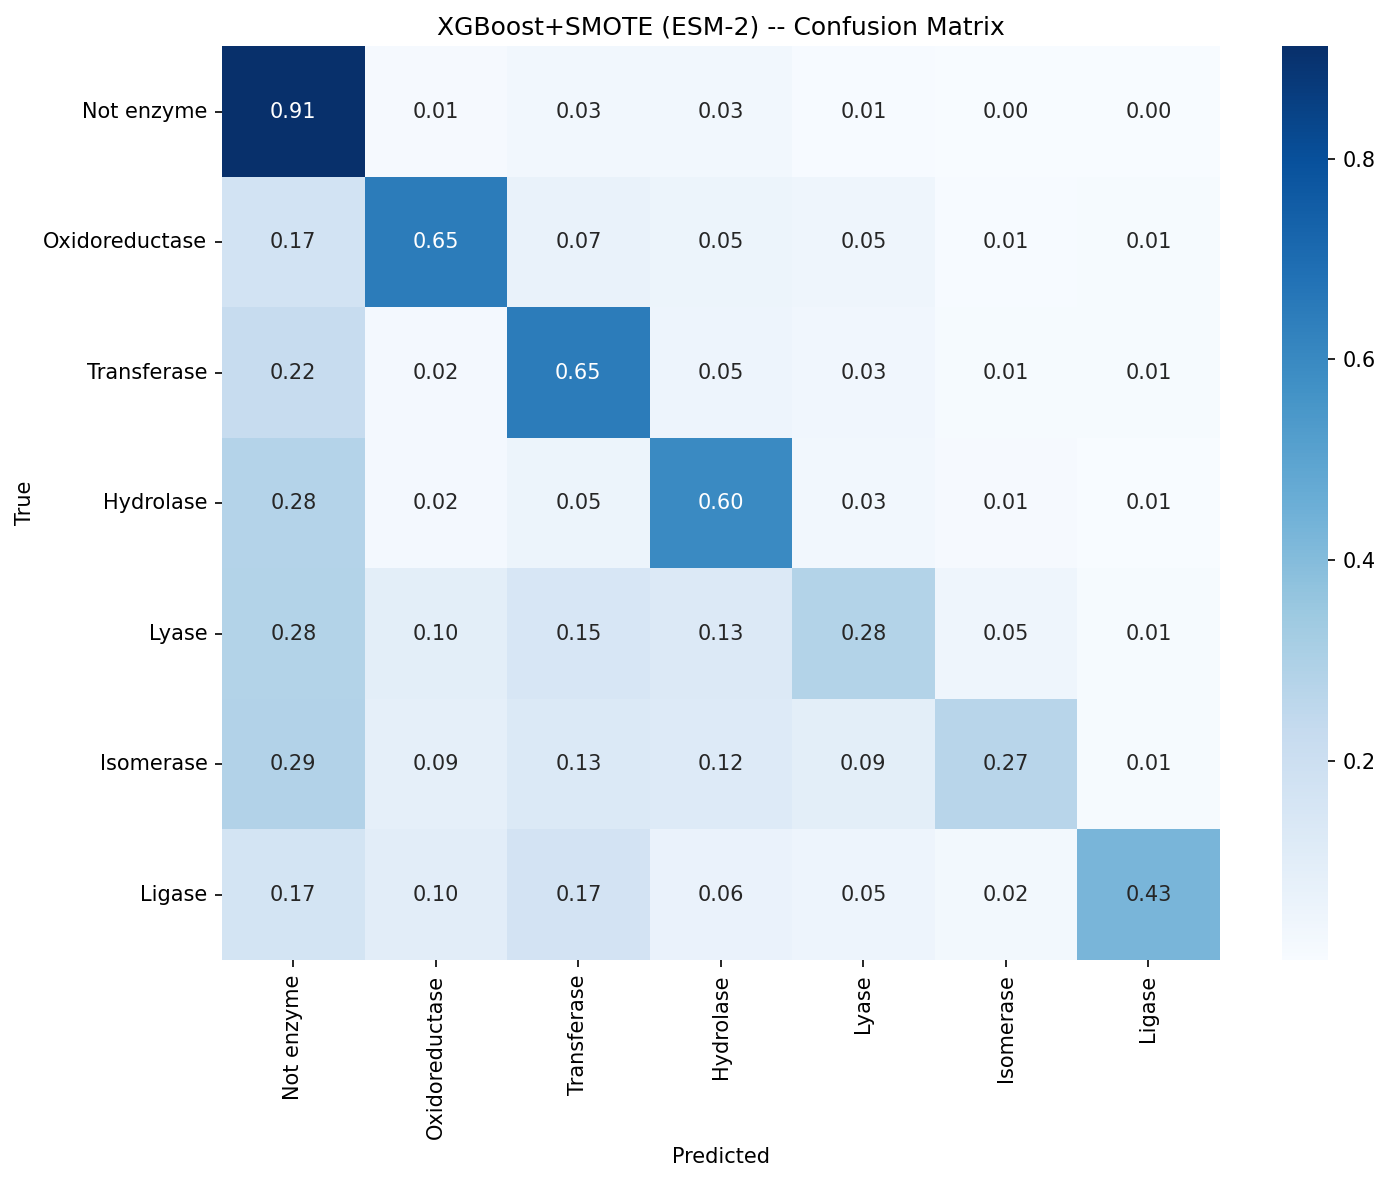
\includegraphics[width=\textwidth]{../figures/cm_xgboost_smote.png}
\caption{Best single model: XGBoost + SMOTE}
\end{subfigure}
\hfill
\begin{subfigure}{0.48\textwidth}
\centering
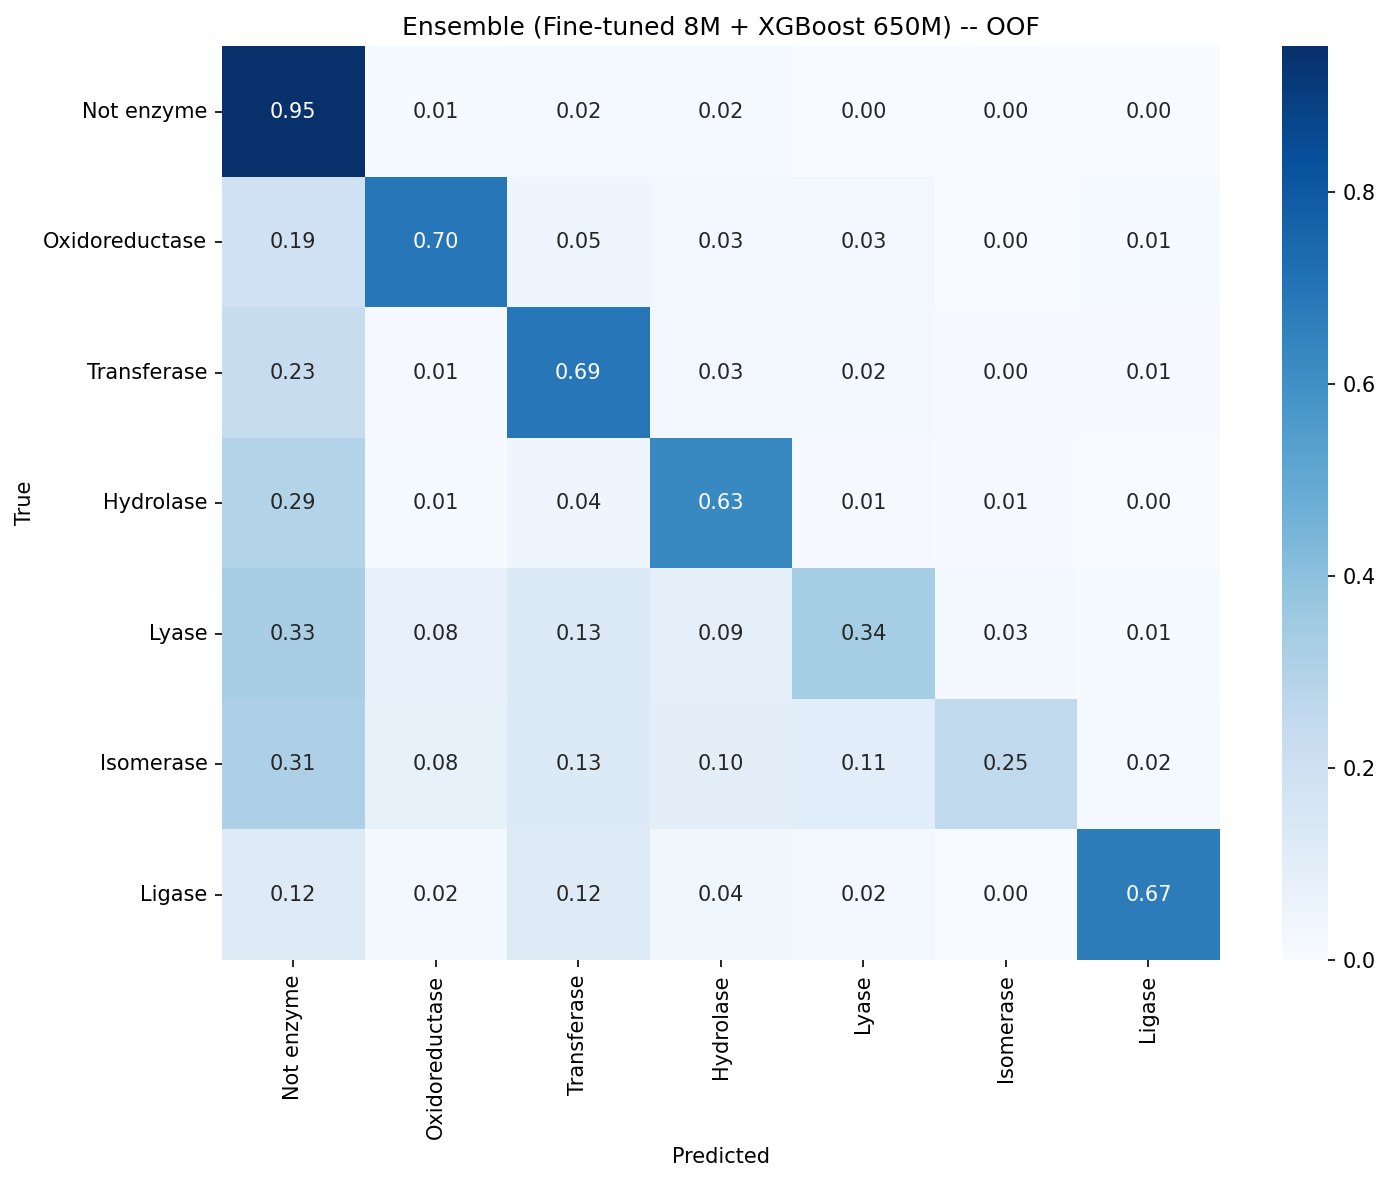
\includegraphics[width=\textwidth]{../figures/cm_ensemble.png}
\caption{Ensemble OOF confusion matrix}
\end{subfigure}
\caption{Row-normalised confusion matrices for top-performing systems.}
\end{figure}

The best single model strongly predicts class 0 (Not enzyme), while Lyase and Isomerase remain
challenging. The ensemble improves overall Macro F1 and Balanced Accuracy through complementary
error patterns between the two constituent models.

\subsection{Confidence Calibration}
\begin{table}[H]
\centering
\caption{Confidence calibration from \texttt{outputs/confidence\_results.json}.}
\begin{tabular}{lccc}
\toprule
Level & Count (\%) & Accuracy & Mean Max Prob \\
\midrule
High ($p \ge 0.80$) & 30448 (76.6\%) & 0.951 & 0.959 \\
Medium ($0.50 \le p < 0.80$) & 6658 (16.7\%) & 0.662 & 0.663 \\
Low ($p < 0.50$) & 2658 (6.7\%) & 0.412 & 0.411 \\
\bottomrule
\end{tabular}
\end{table}

\begin{figure}[H]
\centering
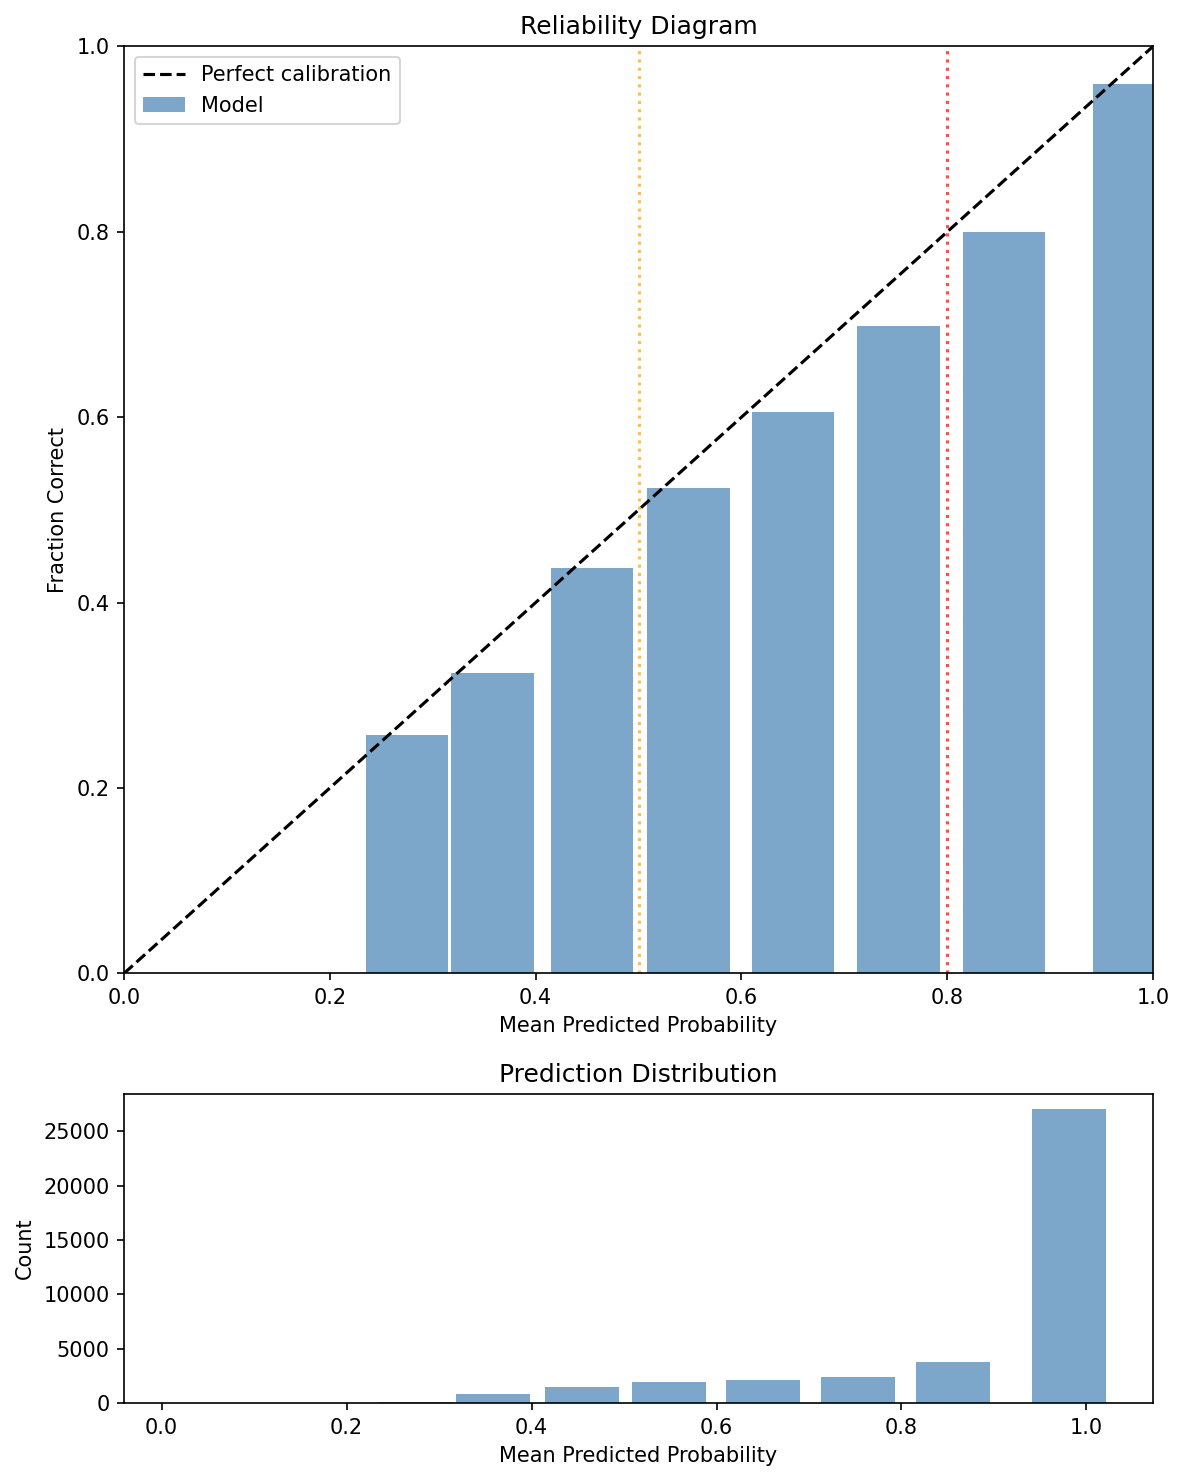
\includegraphics[width=0.72\textwidth]{../figures/reliability_diagram.png}
\caption{Reliability diagram for confidence calibration.}
\end{figure}

\section{Interpretability}
Interpretability was conducted on the best single model (XGBoost + SMOTE).

\textbf{Feature importance.} ESM dimensions dominate top features. The highest-ranked
handcrafted feature is molecular weight.

\textbf{SHAP analysis.} SHAP summary confirms strongest global effects from specific ESM dimensions.

\begin{figure}[H]
\centering
\begin{subfigure}{0.48\textwidth}
\centering
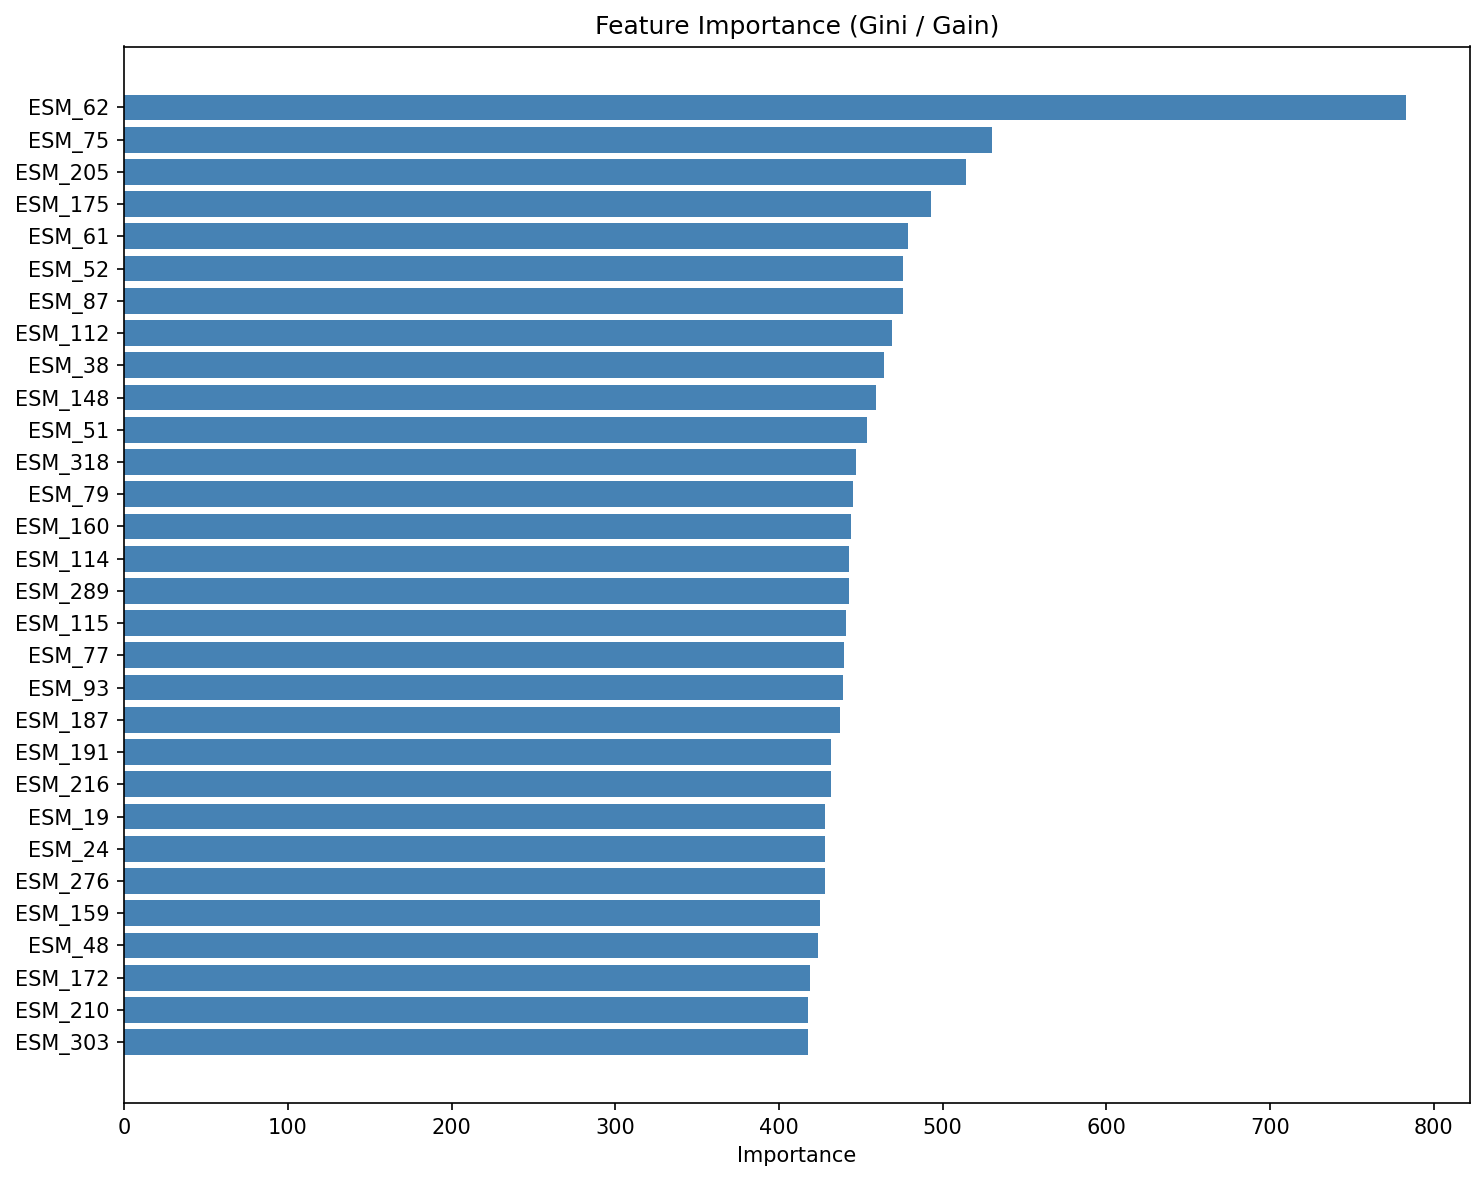
\includegraphics[width=\textwidth]{../figures/feature_importance.png}
\caption{Gini feature importance}
\end{subfigure}
\hfill
\begin{subfigure}{0.48\textwidth}
\centering
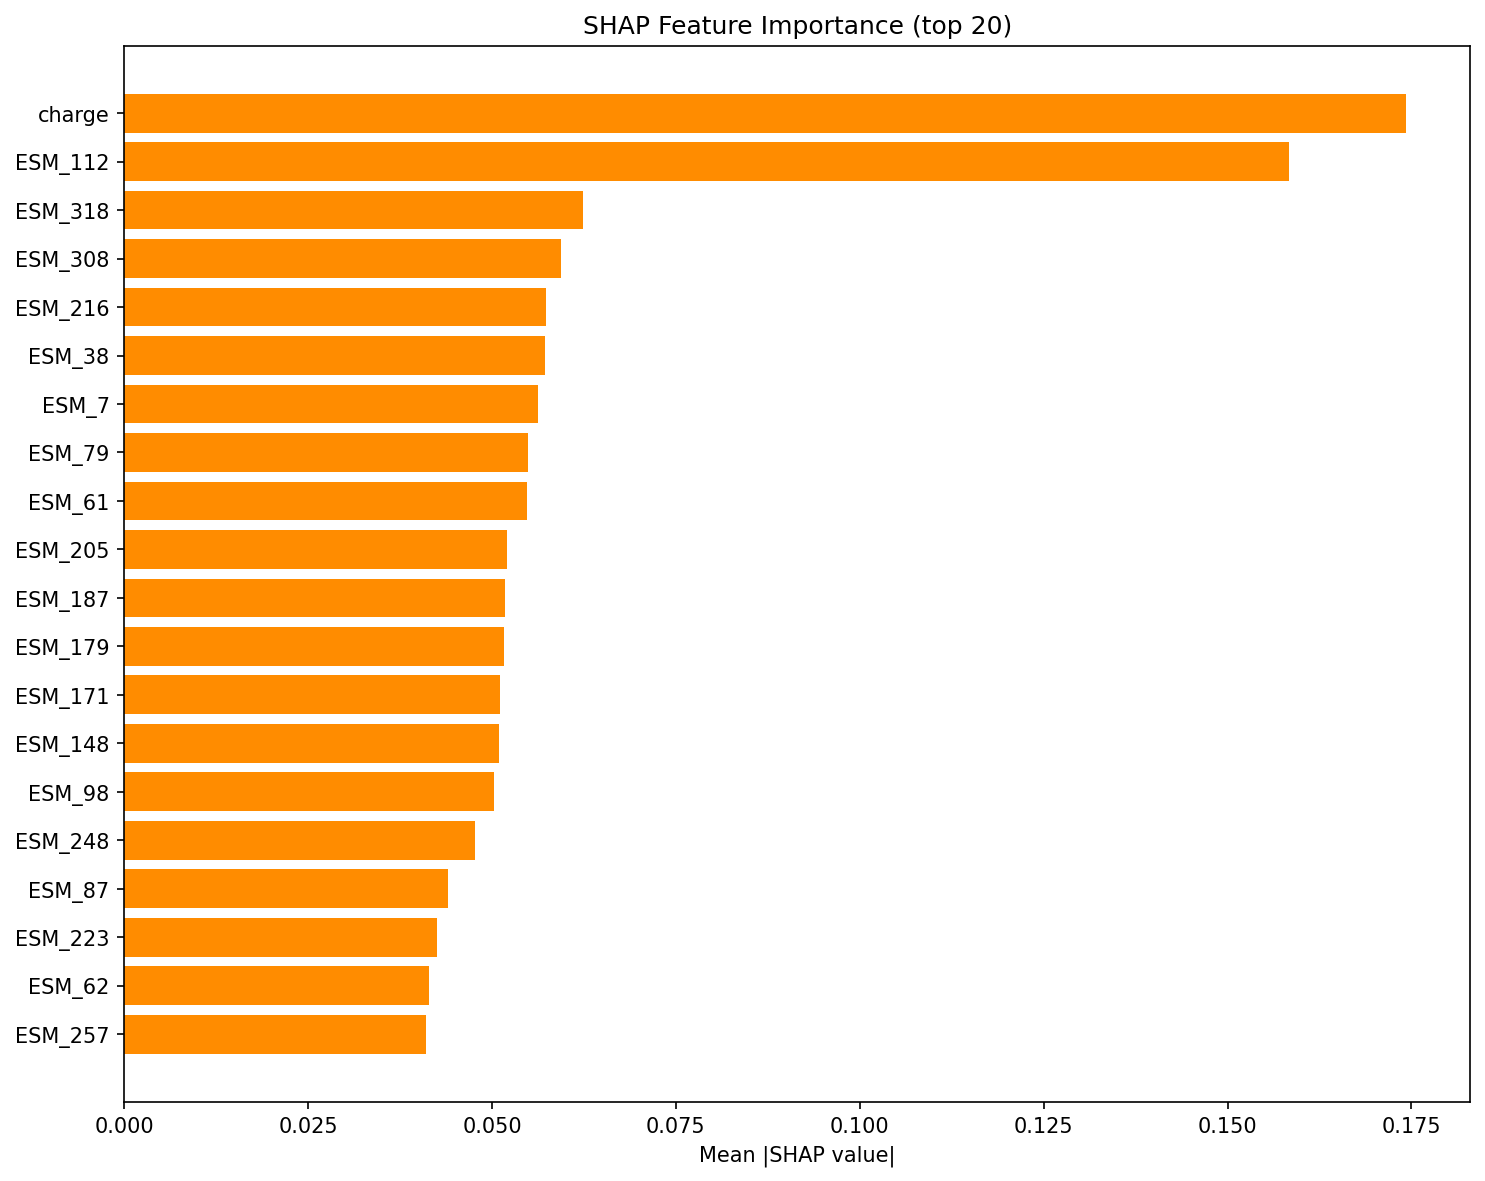
\includegraphics[width=\textwidth]{../figures/shap_importance.png}
\caption{SHAP importance}
\end{subfigure}
\caption{Complementary interpretability views of the best tree-based model.}
\end{figure}

\begin{figure}[H]
\centering
\begin{subfigure}{0.48\textwidth}
\centering
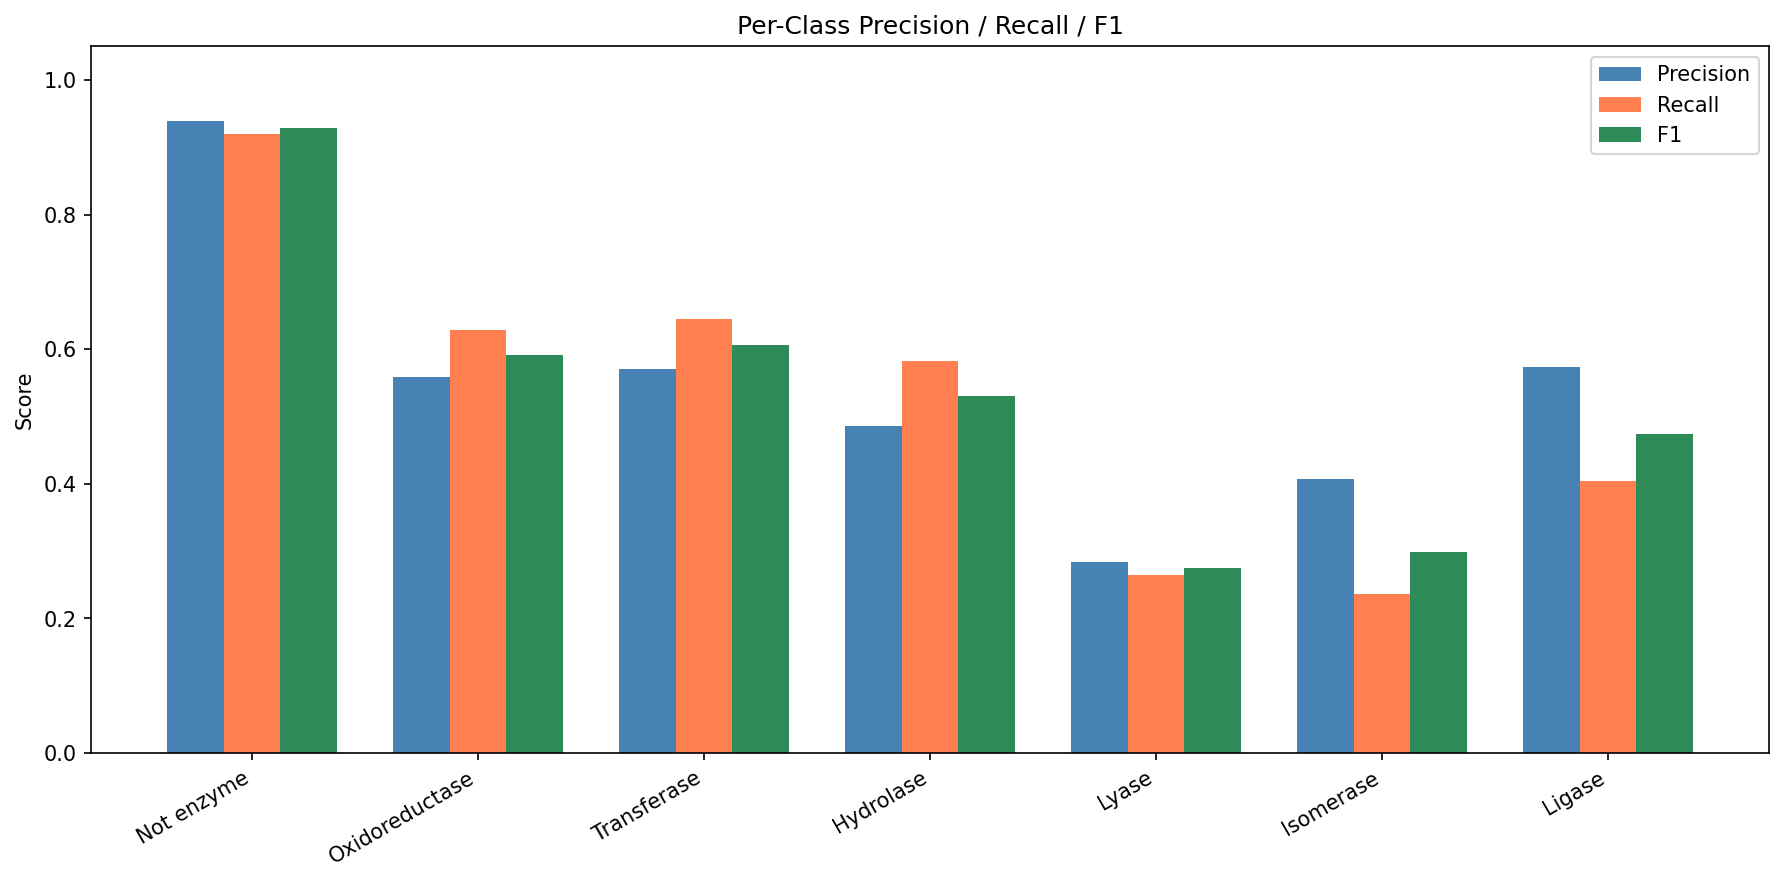
\includegraphics[width=\textwidth]{../figures/per_class_metrics.png}
\caption{Per-class precision/recall/F1}
\end{subfigure}
\hfill
\begin{subfigure}{0.48\textwidth}
\centering
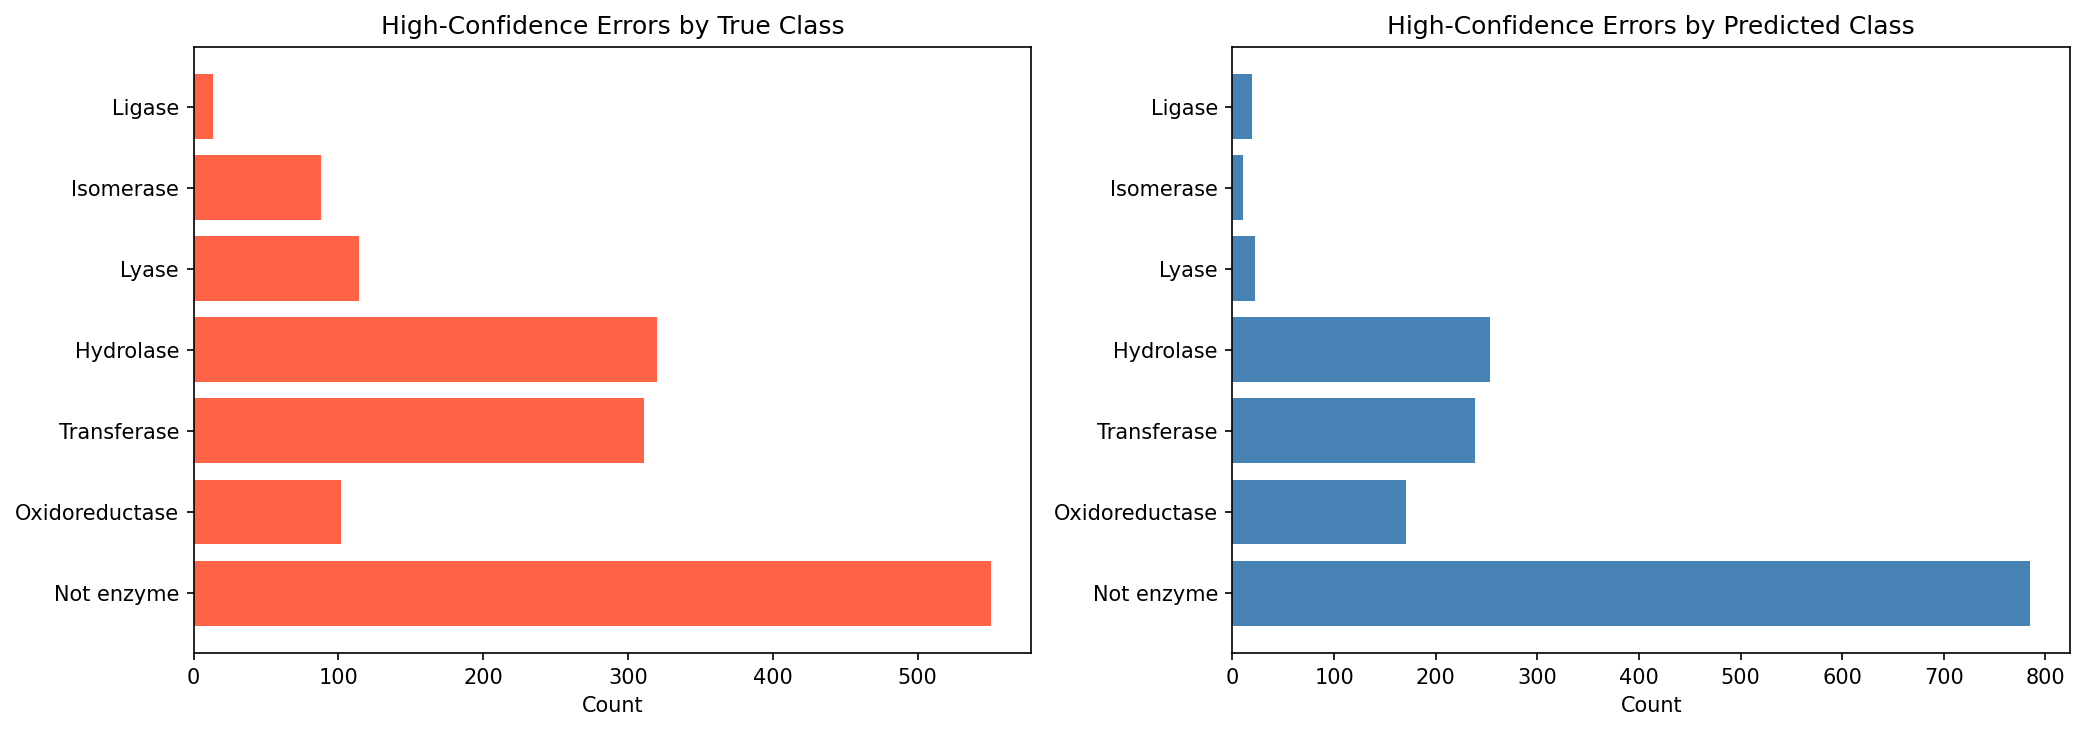
\includegraphics[width=\textwidth]{../figures/high_confidence_errors.png}
\caption{High-confidence error breakdown}
\end{subfigure}
\caption{Class-level behavior and error concentration at high confidence.}
\end{figure}

\begin{table}[H]
\centering
\caption{Per-class metrics for XGBoost + SMOTE (OOF).}
\begin{tabular}{lccc}
\toprule
Class & Precision & Recall & F1 \\
\midrule
Not enzyme & 0.934 & 0.938 & 0.936 \\
Oxidoreductase & 0.586 & 0.629 & 0.607 \\
Transferase & 0.579 & 0.653 & 0.614 \\
Hydrolase & 0.554 & 0.565 & 0.559 \\
Lyase & 0.329 & 0.192 & 0.242 \\
Isomerase & 0.554 & 0.200 & 0.293 \\
Ligase & 0.603 & 0.426 & 0.499 \\
\bottomrule
\end{tabular}
\end{table}

\section{Discussion}
\subsection{What Worked}
The largest gain came from ESM-2 650M embeddings with gradient-boosted trees,
raising Macro F1 from roughly 0.19 to roughly 0.58--0.60.
SMOTE provided a consistent additional lift on minority classes.
The soft-vote ensemble further improved Macro F1 to 0.6247 and MCC to 0.6586.

\subsection{Limitations}
Lyase and Isomerase remain difficult because of limited sample counts.
Fine-tuned ESM-2 8M underperformed frozen 650M embedding-based XGBoost,
likely due to model capacity gap and overfitting risk on the available dataset size.
Adding the full 429-d handcrafted block to ESM-2 features was mildly detrimental.

\subsection{Additional Generated Ensemble Data}
From \texttt{outputs/ensemble\_results.json}:
\begin{itemize}
\item Weight fine-tune: $w_{ft}=0.4608$
\item Weight XGBoost: $w_{xgb}=0.5392$
\item Plain blend Macro F1: 0.6246
\item Optimised-threshold Macro F1: 0.6247
\item Threshold vector approximately unity:
$[1.0000, 0.9999, 0.9999, 0.9999, 1.0000, 0.9999, 0.9999]$
\end{itemize}

\section{Conclusion}
Protein language model representations dominate handcrafted sequence descriptors for this task.
A robust leak-safe CV protocol, explicit imbalance handling, and model ensembling yielded
strong performance on a severely imbalanced 7-class problem.
The final ensemble achieved the best overall trade-off:
\textbf{Accuracy 0.890, Macro F1 0.625, Balanced Accuracy 0.605, MCC 0.659}.

\section{Appendix}
\subsection{Blind Challenge Prediction Command}
\begin{verbatim}
python -m src.predict_blind \
    --fasta <blind_test.fasta> \
    --model outputs/models/best_model.joblib \
    --model-finetune outputs/models/finetune_artifact.joblib \
    --output outputs/predictions/blind_predictions.txt
\end{verbatim}

Output format:
\begin{verbatim}
SEQ01 1 Confidence High
SEQ02 0 Confidence Medium
\end{verbatim}

\subsection{Software Dependencies}
\begin{verbatim}
biopython>=1.83    numpy>=1.26     pandas>=2.1       scikit-learn>=1.4
xgboost>=2.0       lightgbm>=4.2   torch>=2.1        fair-esm>=2.0
matplotlib>=3.8    seaborn>=0.13   shap>=0.44        joblib>=1.3
scipy>=1.12        imbalanced-learn>=0.12             tqdm>=4.66
\end{verbatim}

\subsection{Reproducibility}
All random seeds are fixed to 42 for \texttt{random}, \texttt{numpy}, and \texttt{torch}.
Cross-validation uses stratified 5-fold splitting with shuffling and fixed random state.
Result artifacts are persisted as JSON and reusable model files under \texttt{outputs/}.

\end{document}
